\section{The LVish library interface for application writers}\label{s:lvish-api}

In this section \either{I}{we} illustrate the use of the LVish library
from the point of view of the application writer, through a series of
short example programs.\footnote{Code for all the examples in this
  section is available at
  \url{https://github.com/lkuper/lvar-examples/}.}

\subsection{A simple example: IVars in LVish}

\ifdefined\DISSERTATION

Recall that IVars are data structures that can be shared between
parallel tasks and that allow single writes and blocking reads.
Before looking at LVish, let us consider an IVar computation
implemented with monad-par.

Listing~\ref{listing-ivar-example} shows a program written using
monad-par that will deterministically raise an error, because it tries
to write to the IVar @num@ twice.  Here, @p@ is a computation of type
@Par Int@, meaning that it runs in the @Par@ monad (via the call to
@runPar@) and returns a value of @Int@ type.  @num@ is an IVar,
created with a call to @new@ and then assigned to twice, via two calls
to @put@, each of which runs in a separately @fork@ed task.  The
@runPar@ function is an implicit global barrier: all @fork@s have to
complete before @runPar@ can return.

\singlespacing
\lstinputlisting[float, caption={A basic IVar example using monad-par.}, label=listing-ivar-example]{chapter4/code/ivar-example.hs}
\doublespacing

The code in Listing~\ref{listing-ivar-example} raises a ``multiple
put'' error at runtime, which is as it should be: differing writes to
the same shared location could cause the subsequent call to @get@ to
behave nondeterministically.  Since we are still using monad-par here
and not LVish, @get@ has IVar semantics, not LVar semantics: rather
than performing a threshold read, it blocks until @num@ has been
written, then unblocks and evaluates to the exact contents of @num@.
However, when using monad-par, even multiple writes of the \emph{same}
value to an IVar will raise a ``multiple put'' error, as in
Listing~\ref{listing-repeated-4-ivar}.  This program differs from the
previous one only in that the two @put@s are writing @4@ and @4@,
rather than @3@ and @4@.  Even though the call to @get@ would produce
a deterministic result regardless of which write happened first, the
program nevertheless raises an error because of monad-par's
single-write restriction on IVars.

\singlespacing
\lstinputlisting[float, caption={Repeated writes of the same value to an IVar.}, label=listing-repeated-4-ivar]{chapter4/code/repeated-4-ivar.hs}
\doublespacing

Now let us consider a version of Listing~\ref{listing-repeated-4-ivar}
written using the LVish library. (Of course, in LVish we are not
limited to IVars, but we will consider IVars first as an interesting
special case of LVars, and then go on to consider some more
sophisticated LVars later in this section.)
Listing~\ref{listing-repeated-4-lvar} shows an LVish program that will
write @4@ to an IVar twice and then deterministically print @4@
instead of raising an error.
\fi

\ifdefined\JOURNAL
First, let us consider an LVish program, shown in
Listing~\ref{listing-repeated-4-lvar}, that writes the same value to
an IVar twice.  (Of course, in LVish we are not limited to IVars, but
we will consider IVars first as an interesting special case of LVars,
and then go on to consider some more sophisticated LVars later in this
section.)
\fi

\singlespacing
\lstinputlisting[float, caption={Repeated writes of the same value to an LVar.}, label=listing-repeated-4-lvar]{chapter4/code/repeated-4-lvar.hs}
\doublespacing

\ifdefined\JOURNAL
Compared to a monad-par implementation, the differences in
Listing~\ref{listing-repeated-4-lvar} are minor.
\fi
\either{In Listing~\ref{listing-repeated-4-lvar}, we}{We} need to
import the @Control.LVish@ module rather than @Control.Monad.Par@
(since we now wish to use LVish instead of monad-par), and we must
specifically import @Data.LVar.IVar@ in order to specify which LVar
data structure we want to work with (since we are no longer limited to
IVars).  Just as with monad-par, the LVish @runPar@ function is a
global barrier: both @fork@s must complete before @runPar@ can return.
Also,\either{as before}{as in monad-par}, we have @new@, @put@, and
@get@ operations that respectively create, update, and read from
@num@.  However, these operations now have LVar semantics: the @put@
operation computes a lub (with respect to a lattice similar to that of
Figure~\ref{f:lvars-example-lattices}(b), except including all the
@Int@s), and the @get@ operation performs a threshold read, where the
threshold set is implicitly the set of all @Int@s.  We do not need to
explicitly write down the threshold set in the code.  Rather, it is the
obligation of the @Data.LVar.IVar@ module to provide operations (@put@
and @get@) that have the semantic effect of lub writes and threshold
reads (as \either{I}{we} touched on earlier in
Section~\ref{subsection:lvars-the-model-versus-reality}).

There are two other important differences between \either{the
  monad-par program}{a monad-par implementation} and the LVish
program: the @Par@ type constructor has gained two new type
parameters, @e@ and @s@, and @p@'s type annotation now has a
\emph{type class constraint} of @(HasPut e, HasGet e)@.  Furthermore,
we have added a @LANGUAGE@ pragma, instructing the compiler that we
are now using the @TypeFamilies@ language extension.  In the following
section, \either{I}{we} explain these changes.

\subsection{The \il{e} and \il{s} type parameters: effect tracking and session tracking}

In order to support both deterministic and quasi-deterministic
programming in LVish, we need a way to specify which LVar effects can
occur within a given @Par@ computation.  In a deterministic
computation, only update operations (such as @put@) and threshold
reads should be allowed; in a quasi-deterministic computation,
@freeze@ operations should be allowed as well.  Other combinations may
be desirable as well: for instance, we may want a computation to
perform \emph{only} writes, and not reads.

In order to capture these constraints and make them explicit in the
types of LVar computations, LVish indexes @Par@ computations with a
\emph{phantom type} @e@ that indicates their \emph{effect level}.  The
@Par@ type becomes, instead, @Par e@, where @e@ is a type-level
encoding of Booleans indicating which operations, such as writes,
reads, or freeze operations, are allowed to occur inside it.  LVish
follows the precedent of Kiselyov \etal~on extensible effects in
Haskell~\cite{oleg-amr-haskell-2013}: it abstracts away the specific
structure of @e@ into \emph{type class constraints}, which allow a
@Par@ computation to be annotated with the \emph{interface} that its
@e@ type parameter is expected to satisfy.  This approach allows us to
define ``effect shorthands'' and use them as Haskell type class
constraints.  For example, a @Par@ computation where @e@ is annotated
with the effect level constraint @HasPut@ can perform @put@s.  In our
example above, @e@ is annotated with both @HasPut@ and @HasGet@ and
therefore the @Par@ computation in question can perform both @put@s
and @get@s.  We will see several more examples of effect level
constraints in LVish @Par@ computations shortly.

The effect tracking infrastructure is also the reason why we need to
use the @TypeFamilies@ language extension in our LVish programs.  For
brevity, \either{I}{we} will elide the @LANGUAGE@ pragmas in the rest
of the example LVish programs in this section.

The LVish @Par@ type constructor also has a second type parameter,
@s@, making @Par e s a@ the complete type of a @Par@ computation that
returns a result of type @a@.  The @s@ parameter ensures that, when a
computation in the Par monad is run using the provided @runPar@
operation (or using a variant of @runPar@, which \either{I}{we} will discuss
below), it is not possible to return an LVar from @runPar@ and reuse
it in another call to @runPar@.  The @s@ type parameter also appears
in the types of LVars themselves, and the universal quantification of
@s@ in @runPar@ and its variants forces each LVar to be tied to a
single ``session'', \ie, a single use of a @run@ function, in the same
way that the @ST@ monad in Haskell prevents an @STRef@ from escaping
@runST@.  Doing so allows the LVish implementation to assume that
LVars are created and used within the same session.\footnote{The
  addition of the \il{s} type parameter to \il{Par} in the LVish
  library has nothing to do with LVars in particular; it would also be
  a useful addition to the original \il{Par} library to prevent
  programmers from reusing an IVar from one \il{Par} computation to
  another, which is, as Simon Marlow has noted, ``a Very Bad Idea;
  don't do it''~\cite{marlow-book}.}

\subsection{An observably deterministic shopping cart}\label{subsection:lvish-container-lvars}

\ifdefined\DISSERTATION
\begin{wrapfigure}{r}{1in}
\vspace{-2em}
\begin{center}
  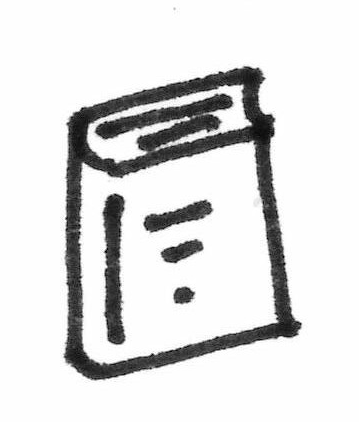
\includegraphics[scale=0.2]{../illustrations/book}
\end{center}
\begin{center}
  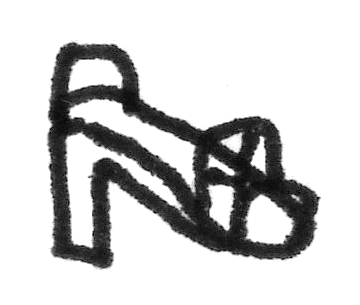
\includegraphics[scale=0.2]{../illustrations/shoe}
\end{center}
\vspace{-3em}
\end{wrapfigure}
\fi

For our next few examples, let us consider concurrently adding items
to a shopping cart.  Suppose we have an @Item@ data type for items
that can be added to the cart.  For the sake of this example, suppose
that only two items are on offer:

\singlespacing
\begin{lstlisting}
data Item = Book | Shoes
  deriving (Show, Ord, Eq)
\end{lstlisting}
\doublespacing

\noindent The cart itself can be represented using the @IMap@ LVar
type (provided by the @Data.LVar.PureMap@\footnote{The ``Pure'' in
  \il{Data.LVar.PureMap} distinguishes it from LVish's other map data
  structure, which is also called \il{IMap}, but is provided by the
  \il{Data.LVar.SLMap} module and is a lock-free data structure based
  on concurrent skip lists.  The \il{IMap} provided by
  \il{Data.LVar.PureMap}, on the other hand, is a reference
  implementation of a map, which uses a pure \il{Data.Map} wrapped in
  a mutable container.  Both \il{IMap}s present the same API, and
  either implementation of \il{IMap} would have worked for this
  example, but the lock-free version is designed to scale as parallel
  resources are added.  \either{I}{We} discuss the role of lock-free
  data structures in LVish in more detail in
  Section~\ref{subsection:lvish-parallel-speedup-results}.} module),
which is a key-value map where the keys are @Item@s and the values are
the quantities of each item.  The name \il{IMap} is by analogy with
\il{IVar}, but here, it is individual entries in the map that are
immutable, not the map itself.  If a key is inserted multiple times,
the values must be equal (according to \il{==}), or a ``multiple put''
error will be raised.

\singlespacing
\lstinputlisting[float, caption={A deterministic shopping-cart program.}, label=listing-map-lvar-getkey-lib]{chapter4/code/map-lvar-getkey-lib.hs}
\doublespacing

Listing~\ref{listing-map-lvar-getkey-lib} shows an LVish program that
inserts items into our shopping cart.  The @newEmptyMap@ operation
creates a new @IMap@, and the @insert@ operation allows us to add new
key-value pairs to the cart.  In this case, we are concurrently adding
the @Book@ item with a quantity of @2@, and the @Shoes@ item with a
quantity of @1@.  The call to @getKey@ will be able to unblock as soon
as the first @insert@ operation has completed, and the program will
deterministically print @2@ regardless of whether the second @insert@
has completed at the time that @getKey@ unblocks.

The @getKey@ operation allows us to threshold on a key---in this case
@Book@---and get back the value associated with that key, once it has
been written.  The (implicit) threshold set of a call to @getKey@ is
the set of all values that might be associated with a key; in this
case, the set of all @Int@s.  This is a legal threshold set because
@IMap@ entries are \emph{immutable}: we cannot, for instance, insert a
key of @Book@ with a quantity of @2@ and then later change the @2@ to
@3@.  In a more realistic shopping cart, the values in the cart could
themselves be LVars representing incrementable counters, as in the
previous section.  However, a shopping cart from which we can
\emph{delete} items is not possible with LVars, because it would go
against the principle of monotonic growth.\footnote{On the other hand,
  one way to implement a container that allows both insertion and
  removal of elements is to represent it internally with \emph{two}
  containers, one for the inserted elements and one for the removed
  elements, where both containers grow monotonically.
  \emph{Conflict-free replicated data types} (CRDTs)~\cite{crdts} use
  variations on this approach to implement various data structures
  that support seemingly non-monotonic operations.  \either{I discuss
    the relationship of LVars to CRDTs in more detail in
    Chapter~\ref{ch:distributed}.}{Bringing these ideas from the
    literature on CRDTs to the setting of LVars is a topic of ongoing
    work~\cite{joining-wodet}.}}

\subsection{A quasi-deterministic shopping cart}

The LVish examples we have seen so far have been fully deterministic;
they do not use @freeze@.  Next, let us consider a program that
freezes and reads the exact contents of a shopping cart, concurrently
with adding items to it.

\singlespacing
\lstinputlisting[float, caption={A quasi-deterministic shopping-cart program.}, label=listing-map-lvar-quasi]{chapter4/code/map-lvar-quasi.hs}
\doublespacing

In Listing~\ref{listing-map-lvar-quasi}, we are @insert@ing items into
our cart, as in Listing~\ref{listing-map-lvar-getkey-lib}.  But,
instead of returning the result of a call to @getKey@, this time @p@
returns the result of a call to @freezeMap@, and the return type of
@p@ is a @Par@ computation containing not an @Int@, but rather an
entire map from @Item@s to @Int@s.  In fact, this map is not the
@IMap@ that @Data.LVar.PureMap@ provides, but rather the standard
@Map@ from the @Data.Map@ module (imported as @M@).  This is possible
because @Data.LVar.PureMap@ is implemented using @Data.Map@, and so
freezing its @IMap@ simply returns the underlying @Data.Map@.

Because @p@ performs a freezing operation, the effect level of its
return type must reflect the fact that it is allowed to perform
freezes.  Therefore, instead of @HasGet@, we have the type class
constraint of @HasFreeze@ on @e@.  Furthermore, because @p@ is allowed
to perform a freeze, we cannot run it with @runPar@, as in our
previous examples, but must instead use a special variant of @runPar@,
called @runParQuasiDet@, whose type signature allows @Par@
computations that allow freezing to be passed to it.

The quasi-determinism in Listing~\ref{listing-map-lvar-quasi} arises
from the fact that the call to @freezeMap@ may run before both
@fork@ed computations have completed.  In this example, one or both
calls to @insert@ may run after the call to @freezeMap@.  If this
happens, the program will raise a write-after-freeze exception.  The
other possibility is that both items are already in the cart at the
time it is frozen, in which case the program will run without error
and print both items.  There are therefore two possible outcomes: a
cart with both items, or a write-after-freeze error.  The advantage of
quasi-determinism is that it is not possible to get multiple
\emph{non-error} outcomes, such as, for instance, an empty cart or a
cart to which only the @Book@ has been added.

\subsection{Regaining full determinism with \il{runParThenFreeze}}\label{subsection:lvish-regaining-full-determinism-with-runparthenfreeze}

The advantage of freezing is that it allows us to observe the exact,
complete contents of an LVar; the disadvantage is that it introduces
quasi-determinism due to the possibility of a write racing with a
freeze, as in the example above.  But, if we could ensure that the
@freeze@ operation happened \emph{last}, we would be able to freeze
LVars with no risk to determinism.  In fact, the LVish library offers
a straightforward solution to this problem: instead of manually
calling @freeze@ (and perhaps accidentally freezing an LVar too
early), we can tell LVish to handle the freezing for us while ``on the
way out'' of a @Par@ computation.  The mechanism that allows this is
another variant of @runPar@, which we call @runParThenFreeze@.

\singlespacing
\lstinputlisting[float, caption={A deterministic shopping-cart program that uses \il{runParThenFreeze}.}, label=listing-map-lvar-freezeafter]{chapter4/code/map-lvar-freezeafter.hs}
\doublespacing

Listing~\ref{listing-map-lvar-freezeafter} shows a version of
Listing~\ref{listing-map-lvar-quasi} written using @runParThenFreeze@.
Unlike the @Par@ computations in the shopping-cart examples we have
seen so far, the @Par@ computation in
Listing~\ref{listing-map-lvar-freezeafter} \emph{only} performs writes
(as we can see from its effect level, which is only constrained by
@HasPut@).  Also, unlike in Listing~\ref{listing-map-lvar-quasi},
where a @freeze@ took place inside the @Par@ computation, in
Listing~\ref{listing-map-lvar-freezeafter} the @Par@ computation
returns an @IMap@ rather than a @Map@.  Since @IMap@ is an LVar, it
has an @s@ parameter, which we can see in the type of @p@.

Because there is no synchronization operation after the two @fork@
calls, @p@ may return @cart@ before both (or either) of the calls to
@insert@ have completed.  However, since @runParThenFreeze@ is an
implicit global barrier (just as @runPar@ and @runParQuasiDet@ are),
both calls to @insert@ \emph{must} complete before @runParThenFreeze@
can return---which means that the result of the program is
deterministic.

\subsection{Event-driven programming with LVars: a deterministic parallel graph traversal}\label{subsection:lvish-parallel-graph-traversal}

Finally, let us look at an example that uses event handlers as well as
freezing.  In Listing~\ref{listing-graph-traversal-explicit-freeze},
the function @traverse@ takes a graph @g@ and a vertex @startNode@ and
finds the set of all vertices reachable from @startNode@, in parallel.
The @traverse@ function first creates a new LVar, called @seen@, to
represent a monotonically growing set of @Int@s that will identify
nodes in the graph.  For this purpose, we use the @ISet@ type,
provided by the @Data.LVar.PureSet@ module.  (As with @IMap@, the
individual elements of the @ISet@ are immutable, but the set itself
can grow.)

\singlespacing
\lstinputlisting[float, caption={A deterministic parallel graph traversal with an explicit call to \il{freeze}.}, label=listing-graph-traversal-explicit-freeze]{chapter4/code/graph-traversal-explicit-freeze.hs}
\doublespacing

Next, @traverse@ attaches an event handler to @seen@.  It does so by
calling the @newHandler@ function, which takes two arguments: an LVar
and the callback that is to be to run every time an event occurs on
that LVar (in this case, every time a new node is added to the
set).\footnote{LVish does not provide \il{newHandler}, but we can
  easily implement it using LVish's built-in \il{newPool} and
  \il{addHandler} operations.}  The callback responds to events by
looking up the neighbors of the newly arrived node (assuming a
@neighbors@ operation, which takes a graph and a vertex and returns a
list of the vertex's neighbor vertices), then mapping the @insert@
function over that list of neighbors.

Finally, @traverse@ adds the starting node to the @seen@ set by
calling @insert startNode seen@---and the event handler does the rest
of the work.  We know that we are done handling events when the call
to @quiesce h@ returns; it will block until all events have been
handled.  Finally, we freeze and return the @ISet@ of all reachable
nodes.  Since @ISet@ is an LVar, it has an @s@ parameter, and in the
return type of @traverse@, the @s@ parameter of @ISet@ has been
replaced by the @Frzn@ type, indicating that the LVar has been frozen.

The good news is that this particular graph traversal program is
deterministic.  The bad news is that, in general, freezing introduces
quasi-determinism, since we could have forgotten to call @quiesce@
before the freeze---which is why @traverse@ must be run with
@runParQuasiDet@, rather than @runPar@.  Although the \emph{program}
is deterministic, the \emph{language-level} guarantee is merely of
quasi-determinism, not determinism.

However, just as with our final shopping-cart example in
Listing~\ref{listing-map-lvar-freezeafter}, we can use
@runParThenFreeze@ to ensure that freezing happens last.
Listing~\ref{listing-graph-traversal-implicit-freeze} gives a version
of @traverse@ that uses @runParThenFreeze@, and eliminates the
possibility of forgetting to call @quiesce@ and thereby introducing
quasi-determinism.

\singlespacing
\lstinputlisting[float, caption={A deterministic parallel graph traversal that uses \il{runParThenFreeze}.}, label=listing-graph-traversal-implicit-freeze]{chapter4/code/graph-traversal-implicit-freeze.hs}
\doublespacing

In Listing~\ref{listing-graph-traversal-implicit-freeze}, since
freezing is performed by @runParThenFreeze@ rather by an explicit call
to @freeze@, it is no longer necessary to constrain @e@ with
@HasFreeze@ in the type of @traverse@.  Furthermore, the @s@ parameter
in the @ISet@ that @traverse@ returns can remain @s@ instead of being
instantiated with @Frzn@.  Most importantly, since freezing is
performed by @runParThenFreeze@ rather by an explicit call to
@freeze@, it is no longer necessary for @traverse@ to explicitly call
@quiesce@, either!  Because of the implicit barrier created by
@runParThenFreeze@, all outstanding events that can be handled will be
handled before it can return.
